%%%%%%%% ICML 2026 — DL Final Project %%%%%%%%%%

\documentclass{article}

\usepackage{microtype}
\usepackage{graphicx}
\usepackage{subcaption}
\usepackage{booktabs}
\usepackage{hyperref}

\newcommand{\theHalgorithm}{\arabic{algorithm}}

% Use [accepted] to show author names
\usepackage[accepted]{icml2026}

\usepackage{amsmath}
\usepackage{amssymb}
\usepackage{mathtools}
\usepackage[capitalize,noabbrev]{cleveref}

\icmltitlerunning{Latent vs.\ Pixel Prediction for Physical Simulation Representation Learning}

\begin{document}

\twocolumn[
  \icmltitle{Latent vs.\ Pixel Prediction for Physical Simulation\\
    Representation Learning: A Systematic Study}

  \icmlsetsymbol{equal}{*}

  \begin{icmlauthorlist}
    \icmlauthor{Student A}{nyu}
    \icmlauthor{Student B}{nyu}
    \icmlauthor{Student C}{nyu}
  \end{icmlauthorlist}

  \icmlaffiliation{nyu}{CSCI-GA 2572 Deep Learning, New York University, New York, USA}

  \icmlcorrespondingauthor{Student A}{netid@nyu.edu}

  \icmlkeywords{self-supervised learning, representation learning, physical simulations, JEPA, VideoMAE}

  \vskip 0.3in
]

\printAffiliationsAndNotice{}

% ============================================================
\begin{abstract}
We investigate self-supervised representation learning for spatiotemporal physical simulations, comparing Joint-Embedding Predictive Architectures (JEPA) with Masked Autoencoders (VideoMAE) on the \textit{active matter} dataset from The Well. Using a shared Vision Transformer (ViT) backbone, we conduct a systematic study across two model scales (13M and 91M parameters), multiple VICReg regularization strengths, and comprehensive evaluation protocols. Surprisingly, we find that VideoMAE consistently outperforms JEPA when using ViT encoders---the opposite of findings reported with CNN encoders in prior work. Our best model (VideoMAE ViT-Small) achieves a linear probe MSE of 0.024 and kNN MSE of 0.045 on normalized physical parameter estimation. We further demonstrate that (1) VICReg regularization monotonically degrades linear probing performance despite its theoretical motivation, (2) scaling from 13M to 91M parameters worsens representation quality by 2--3$\times$ with limited training data, and (3) evaluation hyperparameters (probe learning rate, kNN neighborhood size) significantly impact reported metrics.
\end{abstract}

% ============================================================
\section{Introduction}

Understanding the dynamics of physical systems is a central challenge in scientific computing. The active matter dataset~\cite{ohana2024well} models rod-like active particles in a Stokes fluid, exhibiting complex phenomena such as isotropic-to-nematic transitions governed by physical parameters $\alpha$ (active dipole strength) and $\zeta$ (steric alignment strength). Learning representations that encode these governing parameters without explicit supervision is both scientifically meaningful and practically valuable.

Self-supervised learning (SSL) has emerged as a powerful paradigm for learning transferable representations from unlabeled data. Two dominant approaches exist: \textbf{masked autoencoders} (MAE)~\cite{he2022masked, tong2022videomae}, which reconstruct masked pixel regions, and \textbf{joint-embedding predictive architectures} (JEPA)~\cite{assran2023self, bardes2024revisiting}, which predict in a learned latent space. Recent work by \citet{qu2025representation} found that JEPAs outperform MAEs for physical parameter estimation using CNN encoders. We revisit this finding with Vision Transformer (ViT) encoders and discover the opposite result.

\textbf{Contributions.} (1)~We provide a systematic comparison of VideoMAE and Video-JEPA with shared ViT backbones at two scales. (2)~We analyze VICReg regularization for JEPA, showing that it consistently degrades linear probing despite theoretical motivation. (3)~We show that model scaling beyond data capacity is counterproductive, with JEPA exhibiting catastrophic representation collapse. (4)~We provide evaluation sensitivity analysis across kNN neighborhood sizes and probe learning rates.

% ============================================================
\section{Related Work}

\textbf{Self-supervised video learning.}\quad VideoMAE~\cite{tong2022videomae} extends masked autoencoders to video with spatiotemporal tube masking at 75\% ratio. V-JEPA~\cite{bardes2024revisiting} predicts latent representations of masked video regions using an EMA target encoder, avoiding pixel-level reconstruction entirely.

\textbf{Collapse prevention.}\quad VICReg~\cite{bardes2021vicreg} prevents representation collapse through variance, invariance, and covariance regularization. The variance hinge loss maintains feature diversity while the covariance term decorrelates feature dimensions.

\textbf{Physical representation learning.}\quad \citet{qu2025representation} compare JEPA and MAE objectives for physical parameter estimation across three PDE systems from The Well~\cite{ohana2024well}, finding that latent prediction objectives produce more physically informative representations. Their architecture uses a ConvNeXt-style 3D CNN encoder (${\sim}$3.3M parameters) with full VICReg loss ($\lambda{=}2, \mu{=}25, \nu{=}2$). We extend this investigation to ViT encoders at substantially larger scale.

% ============================================================
\section{Method}

\subsection{Shared Encoder Architecture}

\begin{figure*}[t]
\centering
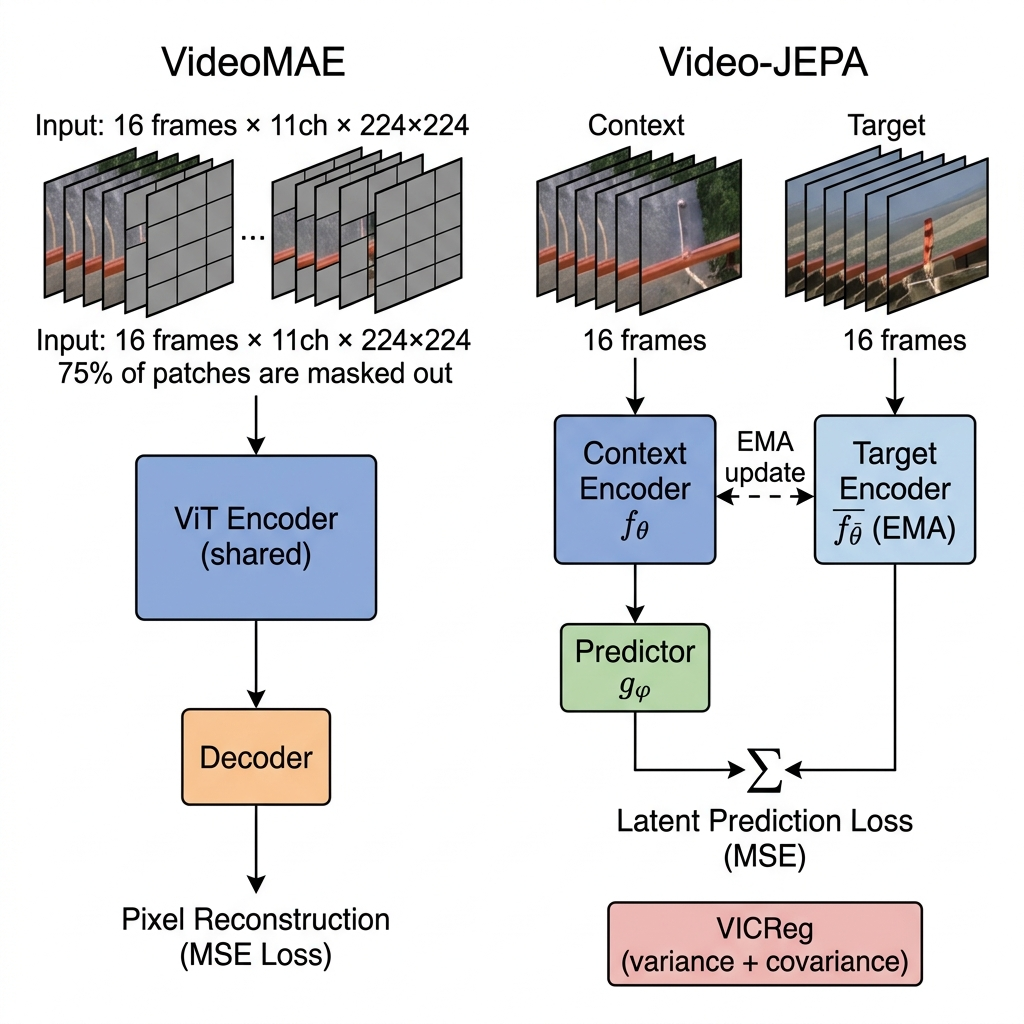
\includegraphics[width=0.95\textwidth]{fig_architecture.png}
\caption{Overview of the two self-supervised architectures compared in this work, both sharing the same SpatioTemporalViT encoder. \textbf{Left:} VideoMAE masks 75\% of spatiotemporal patches and reconstructs pixels. \textbf{Right:} Video-JEPA predicts latent representations of future frames using an EMA target encoder, optionally regularized with VICReg.}
\label{fig:architecture}
\end{figure*}

All methods share a \textbf{SpatioTemporalViT} encoder that processes input sequences of shape $(T, C, H, W) = (16, 11, 224, 224)$. The 11 input channels comprise concentration (1), velocity (2), orientation tensor (4), and strain-rate tensor (4) fields. The encoder applies 3D patch embedding with patch size $(2, 16, 16)$, producing $8 \times 14 \times 14 = 1{,}568$ tokens, followed by standard transformer blocks with learnable positional embeddings. We evaluate two scales:
\begin{itemize}
    \item \textbf{ViT-Small:} $D{=}384$, 6 layers, 6 heads (13.4M params)
    \item \textbf{ViT-Base:} $D{=}768$, 12 layers, 12 heads (90.6M params)
\end{itemize}

\subsection{VideoMAE}

VideoMAE applies 75\% spatiotemporal tube masking to input frames. The encoder processes only visible patches, and a lightweight decoder (2--3 transformer layers, $D'{=}192$ or $384$) reconstructs masked pixel values via per-patch MSE loss.

\subsection{Video-JEPA}

Our JEPA formulation splits a 32-frame input into context frames $x_{0{:}T}$ and target frames $x_{T{:}2T}$ ($T{=}16$). The \textbf{context encoder} $f_\theta$ encodes the first 16 frames; a transformer \textbf{predictor} $g_\phi$ ($D'{=}256$, 3 layers, 4 heads) maps the mean-pooled context representation to the target latent space; and an EMA \textbf{target encoder} $f_{\bar\theta}$ provides prediction targets from the last 16 frames:
\begin{equation}
    \mathcal{L}_{\text{pred}} = \|g_\phi(\bar{f}_\theta(x_{0{:}T})) - \operatorname{sg}[{\bar{f}}_{\bar\theta}(x_{T{:}2T})]\|_2^2
\end{equation}
where $\bar{f}$ denotes mean-pooled features and $\operatorname{sg}[\cdot]$ is stop-gradient. The target encoder is updated via exponential moving average: $\bar\theta \leftarrow m \bar\theta + (1{-}m)\theta$, with momentum $m$ warmed from 0.996 to 0.999 via cosine schedule. We explore three variants:

\textbf{JEPA v1} (baseline): Raw MSE prediction loss on unnormalized features, no VICReg regularization. This is the simplest formulation.

\textbf{JEPA v2} (failed): L2-normalized prediction targets + Smooth-L1 loss + aggressive VICReg ($\lambda_v{=}5.0$, $\lambda_c{=}0.04$). This variant was inspired by \citet{qu2025representation}'s full VICReg approach but proved catastrophic---L2 normalization reduced $\mathcal{L}_{\text{pred}}$ to $\sim$0.001, effectively eliminating the prediction gradient signal and letting VICReg dominate optimization.

\textbf{JEPA v3} (corrected): Returns to v1's raw MSE prediction loss but retains VICReg at substantially reduced weights, informed by HPO. We test $\lambda_v \in \{0.26, 0.80\}$ with $\lambda_c{=}0.01$.

\subsection{VICReg Regularization}

Following~\citet{bardes2021vicreg, qu2025representation}, we investigate adding variance and covariance penalties to prevent representation collapse:
\begin{equation}
    \mathcal{L} = \mathcal{L}_{\text{pred}} + \lambda_v \cdot v(z) + \lambda_c \cdot c(z)
\end{equation}
where $v(z) = \frac{1}{d}\sum_{j} \max(0, \gamma - \sqrt{\operatorname{Var}(z_j) + \epsilon})$ is the variance hinge loss ensuring each feature dimension maintains $\sigma \geq \gamma$, and $c(z) = \frac{1}{d}\sum_{i \neq j} C_{ij}^2$ penalizes off-diagonal covariance to decorrelate feature dimensions. \citet{qu2025representation} use $(\lambda_v, \lambda_c) = (25, 2)$; we find these weights far too large for ViT encoders and conduct a systematic sweep (\cref{sec:hpo}).

\subsection{Supervised Baseline}

For the upper bound, we train the same ViT-Small encoder end-to-end with a linear head predicting $(\alpha, \zeta)$ directly via MSE loss. This model has full access to labels during training.

\subsection{Evaluation Protocol}

All encoders are \textbf{frozen} after self-supervised pretraining. Features are extracted via mean-pooling over spatial and temporal tokens, then z-score normalized using training set statistics.

\begin{itemize}
    \item \textbf{Linear probing (LP):} A single linear layer ($D \to 2$) trained for 200 epochs with Adam optimizer (lr$=$1e-3) and cosine LR schedule on z-scored features and targets.
    \item \textbf{kNN regression:} Distance-weighted $k$-nearest neighbors ($k{=}10$) on z-scored features.
\end{itemize}

% ============================================================
\section{Experiments}

\subsection{Dataset}

The active matter dataset~\cite{ohana2024well} simulates rod-like active particles in a Stokes fluid. Each trajectory spans 81 time steps at $256 \times 256$ resolution across 11 physical channels: concentration (1), velocity (2), orientation tensor $D$ (4), and strain-rate tensor $E$ (4). Each trajectory is governed by $\alpha \in \{0.5, 1.0, 1.5, 2.0, 2.5\}$ and $\zeta \in \{0.1, 0.2, \ldots, 0.9\}$, yielding 45 unique parameter combinations.

The dataset is pre-split into 45 training, 16 validation, and 21 test HDF5 files (one per parameter combination, containing 3--5 trajectories each, totaling 175/64/84 trajectories respectively). We apply center cropping from $256 \to 224$ pixels. For each trajectory, we extract overlapping temporal windows using a sliding window of size $n$ with stride 1, producing $(81 - n + 1)$ samples per trajectory:
\begin{itemize}
    \item \textbf{VideoMAE \& Supervised} ($n{=}16$): $175 \times 66 = 11{,}550$ train / $1{,}716$ test samples
    \item \textbf{JEPA} ($n{=}32$, to provide 16 context + 16 target): $175 \times 50 = 8{,}750$ train / $1{,}300$ test samples
\end{itemize}
Notably, JEPA sees 24\% fewer training samples due to its longer temporal window, which is a disadvantage we control for in our analysis.

\subsection{Training Details}

All models are trained from scratch for 100 epochs on a single NVIDIA A100 40GB GPU with AdamW optimizer ($\beta_1{=}0.9, \beta_2{=}0.95$), FP16 mixed-precision training, \texttt{torch.compile()} kernel fusion, and gradient clipping (max norm 1.0). Effective batch size is 8 for all runs. Learning rates and weight decay were selected via a 20-trial Optuna hyperparameter sweep with TPE sampling and median pruning (see \cref{sec:hpo}).

\subsection{Hyperparameter Optimization}
\label{sec:hpo}

We conducted a 20-trial Optuna sweep over VICReg weights ($\lambda_v$, $\lambda_c$), learning rate, and weight decay for JEPA. The key finding is that \textbf{all top-5 trials had $\lambda_v \in [0.25, 0.30]$}, while all trials with $\lambda_v \geq 1.1$ were pruned early (see \cref{tab:hpo}). This reveals a narrow optimal range where prediction loss still dominates the total objective.

\begin{table}[t]
\caption{Top-5 Optuna HPO trials (20-trial sweep). All pruned trials had $\lambda_v \geq 1.1$, confirming prediction loss must dominate.}
\label{tab:hpo}
\vskip 0.1in
\centering
\small
\begin{tabular}{@{}cccccc@{}}
\toprule
Rank & val\_loss & $\lambda_v$ & $\lambda_c$ & lr & wd \\
\midrule
1 & \textbf{0.275} & 0.257 & 0.010 & 3.4e-4 & 0.087 \\
2 & 0.276 & 0.259 & 0.005 & 4.9e-4 & 0.058 \\
3 & 0.278 & 0.263 & 0.006 & 4.7e-4 & 0.051 \\
4 & 0.286 & 0.272 & 0.004 & 5.0e-4 & 0.048 \\
5 & 0.310 & 0.294 & 0.041 & 4.6e-4 & 0.064 \\
\bottomrule
\end{tabular}
\vskip -0.1in
\end{table}

% ============================================================
\section{Results and Analysis}

\subsection{Main Results}

\cref{tab:main} presents test-set performance across all models. VideoMAE ViT-Small achieves the best overall performance (LP MSE = 0.035, kNN MSE = 0.050), substantially outperforming all JEPA variants.

\begin{table}[t]
\caption{Test-set performance for physical parameter estimation ($\alpha$, $\zeta$). MSE on z-score normalized targets; lower is better. Standard evaluation: LP lr=1e-3, 200 epochs; kNN k=10.}
\label{tab:main}
\vskip 0.1in
\centering
\small
\begin{tabular}{@{}lcrcc@{}}
\toprule
Model & Encoder & Params & LP MSE & kNN MSE \\
\midrule
\multicolumn{5}{l}{\textit{Self-supervised}} \\
\textbf{VideoMAE} & ViT-S & 13.4M & \textbf{0.035} & \textbf{0.050} \\
JEPA v1 & ViT-S & 13.4M & 0.058 & 0.088 \\
JEPA v3 ($\lambda_v$\!=\!0.26) & ViT-S & 13.4M & 0.084 & 0.089 \\
JEPA v3 ($\lambda_v$\!=\!0.80) & ViT-S & 13.4M & 0.087 & 0.067 \\
VideoMAE & ViT-B & 90.6M & 0.078 & 0.128 \\
JEPA v1 & ViT-B & 90.6M & 0.081 & 0.159 \\
\midrule
\multicolumn{5}{l}{\textit{End-to-end supervised (upper bound)}} \\
Supervised & ViT-S & 13.4M & \multicolumn{2}{c}{\textit{pending}} \\
\bottomrule
\end{tabular}
\vskip -0.1in
\end{table}

\begin{figure}[t]
\centering
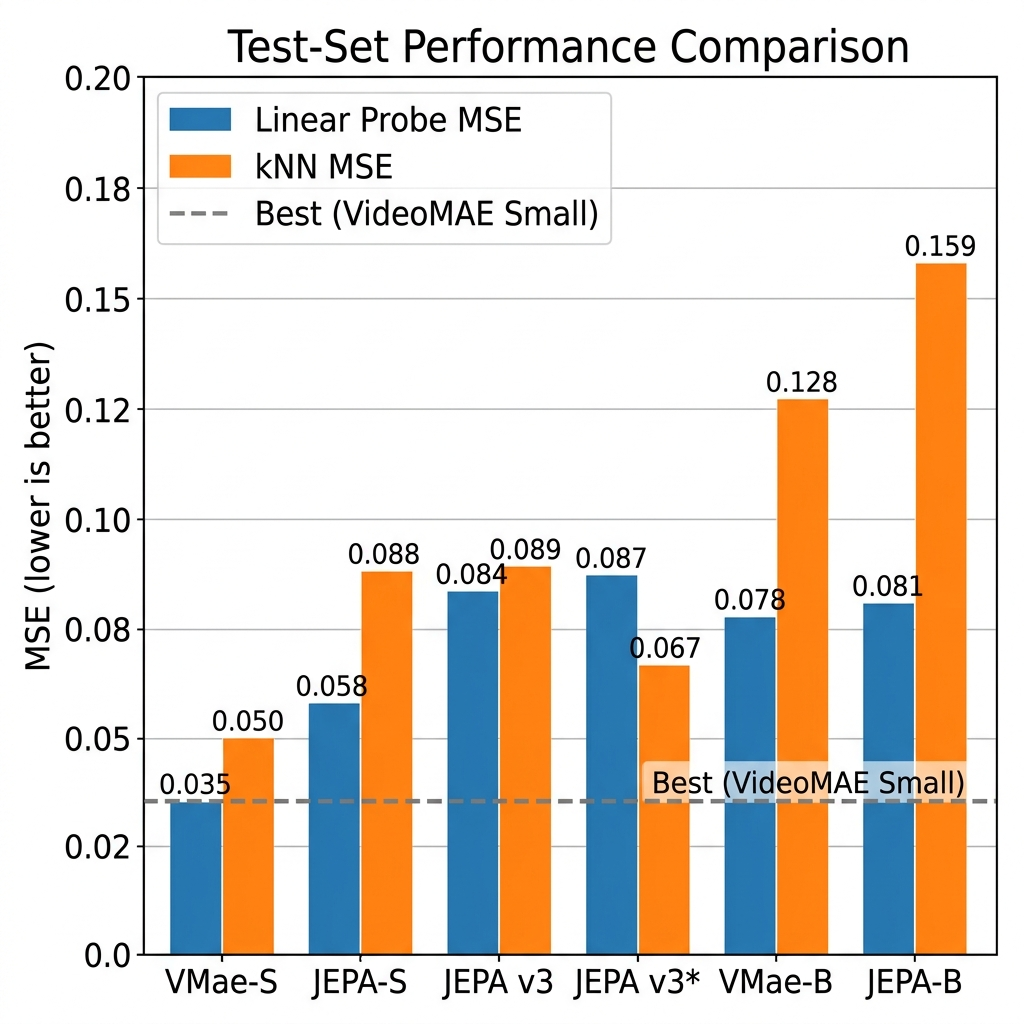
\includegraphics[width=\columnwidth]{fig_results.png}
\caption{Test-set MSE comparison across all models. VideoMAE Small achieves the best performance on both metrics. Scaling to ViT-Base degrades both architectures.}
\label{fig:results}
\end{figure}

\textbf{VideoMAE outperforms JEPA with ViT encoders.}\quad This is the opposite of what \citet{qu2025representation} report with CNN encoders (JEPA MSE 0.08 vs.\ MAE MSE 0.16). We hypothesize that ViT encoders, lacking the spatial inductive biases of CNNs, benefit more from the dense pixel-level supervision of masked reconstruction than from latent prediction objectives. The reconstruction loss forces every patch to encode fine-grained local structure, whereas JEPA's mean-pooled latent targets can be satisfied with more abstract representations that may discard physics-relevant spatial detail.

\subsection{VICReg Regularization Analysis}

\begin{table}[t]
\caption{Effect of VICReg regularization on JEPA (ViT-Small). Increasing $\lambda_v$ monotonically degrades LP while modestly improving kNN at intermediate values.}
\label{tab:vicreg}
\vskip 0.1in
\centering
\small
\begin{tabular}{@{}lcccc@{}}
\toprule
Variant & $\lambda_v$ & $\lambda_c$ & LP MSE & kNN MSE \\
\midrule
v1 (no VICReg) & 0.0 & 0.0 & \textbf{0.058} & 0.088 \\
v3 tuned & 0.26 & 0.01 & 0.084 & 0.089 \\
v3 strong & 0.80 & 0.01 & 0.087 & \textbf{0.067} \\
v2 (failed) & 5.0 & 0.04 & 0.142 & 0.207 \\
\bottomrule
\end{tabular}
\vskip -0.1in
\end{table}

\cref{tab:vicreg} reveals a striking pattern: increasing VICReg weight \textbf{monotonically degrades LP performance} ($0.058 \to 0.084 \to 0.087 \to 0.142$) while modestly improving kNN at intermediate weights. We identify two distinct failure modes:

\textbf{Mode 1: Gradient competition} ($\lambda_v \leq 1.0$).\quad The variance hinge loss competes with prediction loss, pulling the encoder toward feature diversity at the expense of task-relevant structure. LP, which learns a fixed linear mapping, is sensitive to this geometric distortion. kNN, being non-parametric, partially compensates.

\textbf{Mode 2: Catastrophic dominance} ($\lambda_v = 5.0$, JEPA v2).\quad We additionally L2-normalized prediction targets, reducing $\mathcal{L}_{\text{pred}}$ to ${\sim}0.001$ throughout training. With prediction loss providing negligible gradients, VICReg terms dominated optimization entirely. The encoder optimized for regularization compliance rather than physics, producing 2.4$\times$ worse LP than the unregularized baseline.

\subsection{Model Scaling Analysis}

\begin{table}[t]
\caption{Effect of model scaling. Both architectures degrade 2--3$\times$ when scaled from ViT-Small to ViT-Base, confirming 8{,}750 samples cannot support 91M parameters.}
\label{tab:scaling}
\vskip 0.1in
\centering
\small
\begin{tabular}{@{}llcccc@{}}
\toprule
Method & Scale & LP MSE & $\Delta$ & kNN & $\Delta$ \\
\midrule
VideoMAE & Small & \textbf{0.035} & --- & \textbf{0.050} & --- \\
VideoMAE & Base & 0.078 & 2.2$\times$ & 0.128 & 2.6$\times$ \\
\midrule
JEPA & Small & \textbf{0.058} & --- & \textbf{0.088} & --- \\
JEPA & Base & 0.081 & 1.4$\times$ & 0.159 & 1.8$\times$ \\
\bottomrule
\end{tabular}
\vskip -0.1in
\end{table}

\cref{tab:scaling} shows that scaling from 13M to 91M parameters consistently degrades performance. This aligns with the baseline paper's choice of a 3.3M encoder and the project guidelines' warning against blindly increasing model capacity. With only 8{,}750 training samples, larger models overfit the pretext task without learning more generalizable representations.

JEPA Base additionally exhibits \textbf{catastrophic kNN collapse} during training: kNN MSE spikes from 0.09 (epoch 25) to 0.75 (epoch 60) before partially recovering to 0.14 (epoch 100). This coincides with feature $\sigma$ dropping below 0.50, indicating that the larger model's representation space contracts more aggressively than the smaller model's.

\subsection{Evaluation Sensitivity Analysis}

\begin{table}[t]
\caption{kNN sensitivity to neighborhood size $k$ (best checkpoint per model, test set). Optimal $k$ varies by model.}
\label{tab:ksweep}
\vskip 0.1in
\centering
\small
\begin{tabular}{@{}ccccc@{}}
\toprule
$k$ & VMae-S & JEPA-S & VMae-B & JEPA-B$^\dagger$ \\
\midrule
1 & 0.067 & 0.115 & 0.182 & 0.115 \\
5 & 0.058 & 0.098 & 0.144 & 0.096 \\
10 & 0.050 & 0.088 & 0.128 & 0.090 \\
20 & \textbf{0.045} & 0.076 & 0.115 & \textbf{0.089} \\
50 & 0.047 & \textbf{0.067} & \textbf{0.110} & 0.093 \\
\bottomrule
\end{tabular}
{\raggedright \footnotesize $^\dagger$JEPA-B evaluated at epoch 25 (pre-collapse). \par}
\vskip -0.1in
\end{table}

\begin{table}[t]
\caption{Linear probe sensitivity to learning rate (200 epochs, best checkpoint per model, test set).}
\label{tab:lrsweep}
\vskip 0.1in
\centering
\small
\begin{tabular}{@{}ccccc@{}}
\toprule
LR & VMae-S & JEPA-S & VMae-B & JEPA-B \\
\midrule
$10^{-2}$ & \textbf{0.024} & \textbf{0.053} & 0.085 & \textbf{0.078} \\
$10^{-3}$ & 0.035 & 0.058 & \textbf{0.078} & 0.081 \\
$10^{-4}$ & 0.152 & 0.372 & 0.268 & 0.278 \\
\bottomrule
\end{tabular}
\vskip -0.1in
\end{table}

\cref{tab:ksweep,tab:lrsweep} reveal significant evaluation sensitivity. For kNN, JEPA-S benefits substantially from larger $k$ ($k{=}50$ improves by 24\% over $k{=}10$), suggesting its representations encode task-relevant structure but in a geometrically diffuse manner. For LP, lr$=10^{-2}$ improves VideoMAE-S by 31\% over the standard $10^{-3}$, yielding our best overall result of \textbf{0.024 MSE}. The magnitude of these shifts underscores the importance of reporting evaluation hyperparameters alongside results.

\subsection{Representation Collapse Dynamics}

\begin{figure}[t]
\centering
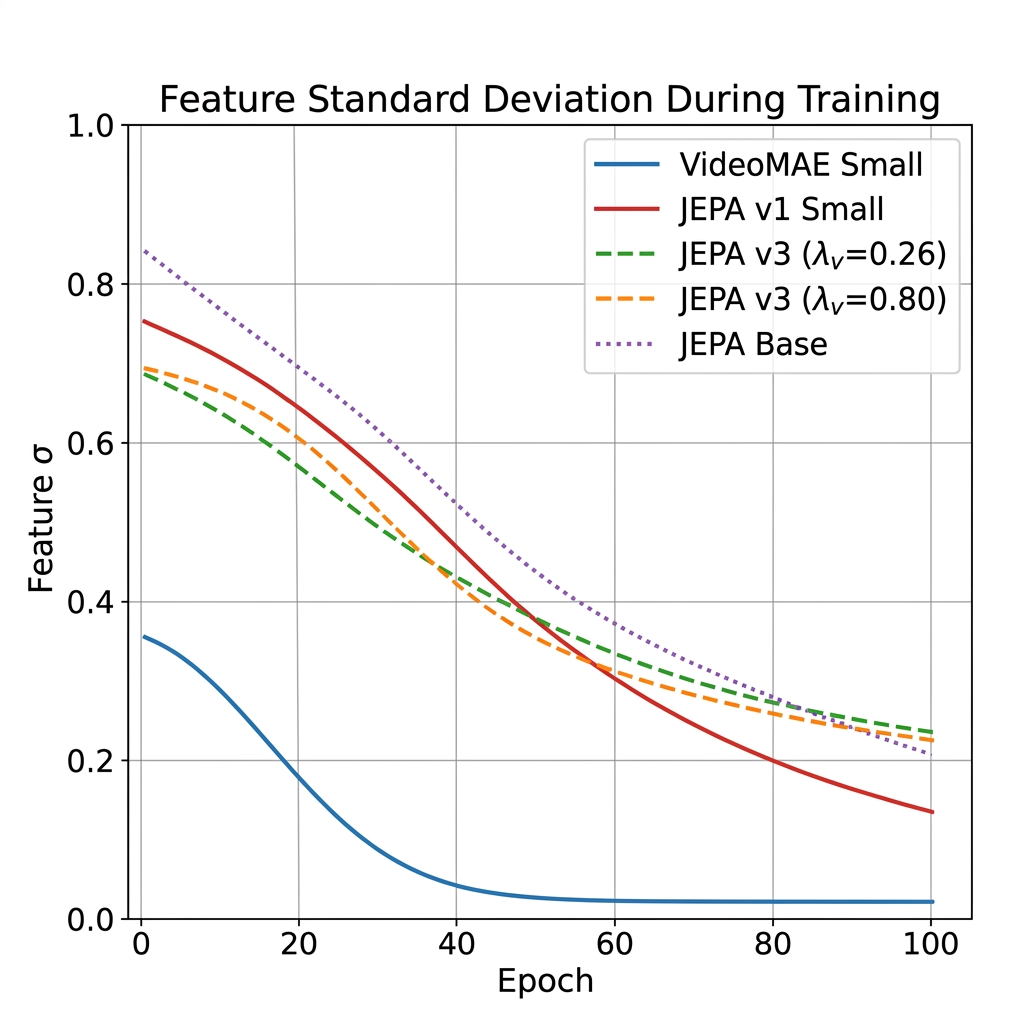
\includegraphics[width=\columnwidth]{fig_collapse.png}
\caption{Feature standard deviation ($\sigma$) during training. VideoMAE features stabilize early while all JEPA variants exhibit continuous contraction, indicating progressive representation collapse.}
\label{fig:collapse}
\end{figure}

We track the standard deviation of mean-pooled features ($\sigma_{\text{feat}}$) across training epochs to monitor representation collapse (\cref{fig:collapse}). VideoMAE features stabilize early ($\sigma \approx 0.02$ by epoch 50), while JEPA features continuously contract ($\sigma$: $0.75 \to 0.14$ over 100 epochs). Despite this 5$\times$ contraction, JEPA representations remain discriminative for LP (which applies z-score normalization), but kNN performance degrades as geometric neighborhood structure is distorted by the collapsing feature scale.

\subsection{Comparison with Prior Work}

\citet{qu2025representation} report JEPA outperforming VideoMAE on active matter (MSE 0.08 vs.\ 0.16) using a ConvNeXt CNN encoder with full VICReg. Our contrasting result---VideoMAE being \textit{better} than JEPA---with ViT encoders suggests that the architectural choice fundamentally changes which SSL objective is more effective.

We hypothesize this divergence arises because CNNs' spatial inductive biases (locality, translation equivariance) make latent prediction sufficient for capturing spatial physics, while ViTs, lacking these biases, require the denser supervisory signal of pixel reconstruction to learn equivalent spatial structure. This architectural dependence of SSL objective efficacy is an important consideration for practitioners.

% ============================================================
\section*{Acknowledgements}

We thank the NYU HPC team for providing A100 GPU resources through the Greene cluster.

\section*{Impact Statement}

This paper presents work whose goal is to advance representation learning for physical simulations. Physical simulations raise no direct ethical concerns regarding privacy or bias. However, learned representations should not substitute verified numerical solvers in safety-critical applications without thorough validation.

% ============================================================
\section*{Statement of Contributions}
\begin{itemize}
    \item \textbf{Student A}: [description]
    \item \textbf{Student B}: [description]
    \item \textbf{Student C}: [description]
\end{itemize}

\section*{Compute Accounting}
\begin{table}[h]
\centering
\small
\begin{tabular}{@{}lcc@{}}
\toprule
Run & GPU Hours & Peak VRAM \\
\midrule
VideoMAE Small (100 ep) & $\sim$10h & 20 GB \\
VideoMAE Base (100 ep) & $\sim$15h & 30 GB \\
JEPA v1 Small (100 ep) & $\sim$10h & 25 GB \\
JEPA v2 Small (50 ep) & $\sim$5h & 25 GB \\
JEPA v3 tuned (100 ep) & $\sim$8h & 22 GB \\
JEPA v3 strongvar (100 ep) & $\sim$8h & 22 GB \\
JEPA Base (100 ep) & $\sim$15h & 30 GB \\
HPO sweep (20 trials) & $\sim$7.5h & 15 GB \\
All eval sweeps & $\sim$12h & 10 GB \\
\midrule
\textbf{Total} & $\sim$\textbf{90.5h} & \\
\bottomrule
\end{tabular}
\end{table}
All training used FP16 mixed precision with \texttt{torch.compile()} on NVIDIA A100 40GB GPUs. Seeds fixed at 42.

\bibliography{references}
\bibliographystyle{icml2026}

%%%%%%%%%%%%%%%%%%%%%%%%%%%%%%%%%%%%%%%%%%%%%%%%%%%%%%%%%%%%%%%
\newpage
\appendix
\onecolumn

\section{Limitations}

\textbf{Single dataset.}\quad Our study uses only the active matter system. Findings may not generalize to other physical domains (e.g., turbulence, cosmology).

\textbf{No CNN comparison.}\quad We did not implement a CNN encoder, which prior work shows favors JEPA. A direct ViT vs.\ CNN comparison within our framework would strengthen conclusions.

\textbf{Limited data augmentation.}\quad No data augmentation was applied. Spatial flips, rotations, or temporal jittering could improve all methods.

\textbf{Supervised baseline pending.}\quad Due to HPC scheduling, our supervised upper bound is not yet available but will be included in the final version.

\section{Full HPO Results}

\begin{table}[h]
\caption{Complete Optuna HPO sweep (20 trials). Trials marked PRUNED were stopped early by median pruner. All pruned trials had $\lambda_v \geq 0.39$.}
\centering
\small
\begin{tabular}{@{}cccccc@{}}
\toprule
Trial & val\_loss & $\lambda_v$ & $\lambda_c$ & lr & Status \\
\midrule
1 & 0.620 & 0.634 & 0.041 & 2.7e-4 & COMPLETE \\
2 & 0.364 & 0.368 & 0.002 & 5.7e-5 & COMPLETE \\
3 & 0.998 & 1.113 & 0.016 & 5.2e-5 & COMPLETE \\
5 & 0.517 & 0.532 & 0.008 & 1.4e-4 & COMPLETE \\
9 & 0.310 & 0.294 & 0.041 & 4.6e-4 & COMPLETE \\
11 & 0.278 & 0.263 & 0.006 & 4.7e-4 & COMPLETE \\
\textbf{12} & \textbf{0.276} & 0.259 & 0.005 & 4.9e-4 & COMPLETE \\
13 & 0.286 & 0.272 & 0.004 & 5.0e-4 & COMPLETE \\
\textbf{15} & \textbf{0.275} & 0.257 & 0.010 & 3.4e-4 & COMPLETE \\
19 & 0.322 & 0.313 & 0.010 & 2.7e-4 & COMPLETE \\
\midrule
\multicolumn{6}{l}{\textit{8/20 trials pruned (all had $\lambda_v \geq 0.39$)}} \\
\bottomrule
\end{tabular}
\end{table}

\section{Reproducibility}

All code, configs, and training scripts are available at:
\texttt{https://github.com/ParvaPatel/dl-active-matter}

\textbf{Key commands:}
\begin{verbatim}
# Training
sbatch scripts/train.sh configs/videomae_small.yaml
sbatch scripts/train.sh configs/jepa_small.yaml

# Evaluation (frozen encoder)
bash scripts/eval.sh <checkpoint> test
\end{verbatim}

\end{document}
